\documentclass{article}
\usepackage{rapport}

\title{Projet Systèmes d'Exploitation -- Jeu Sherlock 13}
\author{Xiaochen YANG\\21419435}
\date{}

\begin{document}

\maketitle

\section*{Introduction}

Ce rapport décrit la mise en œuvre d'une version graphique Web du jeu Sherlock 13. Ce projet est un programme développé 
en langage C utilisant le protocole TCP pour permettre à quatre joueurs de jouer les uns contre les autres sur le réseau, et utilise la bibliothèque SDL2 pour implémenter l'interface graphique.

\section{Construction du programme}

Le projet était fourni sous forme d'un squelette avec deux fichiers principaux, \texttt{server\_logic.c} pour le serveur et \texttt{client\_logic.c} pour le client.
Plusieurs fichiers secondaires \texttt{gui.c}, \texttt{resources.c}, etc., étaient également présents pour la partie graphique. 
Il a d'abord été nécessaire d'analyser la structure existante pour identifier les fonctions à implémenter.

\subsection{Partie serveur}

Le serveur accepte les connexions des clients grâce à des sockets TCP, configurés avec les appels classiques pour créer, attacher et écouter sur un port réseau. 
Lorsqu'un client se connecte, le serveur lui dédie un thread indépendant qui prend en charge ses échanges, ce qui permet de gérer plusieurs joueurs en même temps.

Pour cela, le programme utilise une structure de données qui regroupe les informations de chaque joueur, 
comme son adresse IP, son port d'écoute ou encore le nom qu'il a choisi. Une autre structure garde la répartition des cartes et les symboles que chaque joueur possède. 
Les cartes sont mélangées de manière aléatoire, puis attribuées aux joueurs. À partir de ces cartes, on calcule combien de fois chaque symbole est présent chez chaque joueur.

Quand un joueur effectue une action (observer un symbole, poser une question à un autre joueur, accuser quelqu'un), 
le serveur lit le message reçu, en extrait les informations nécessaires, met à jour l'état du jeu si besoin, 
puis envoie une réponse à tous les joueurs connectés. Cette communication permet à tous de rester synchronisés sur le déroulement de la partie.

La logique du serveur permet de gérer jusqu'à quatre participants. 
Chaque joueur reçoit un identifiant unique, et un port de communication est ouvert pour chaque fil. 
Le serveur distribue les cartes, annonce les changements de tour, et détermine si un joueur gagne ou est éliminé, en tenant compte des règles du jeu. 
Chaque événement est transmis à tous les clients pour qu'ils puissent mettre à jour leur interface.

\begin{figure}[H]
    \centering
    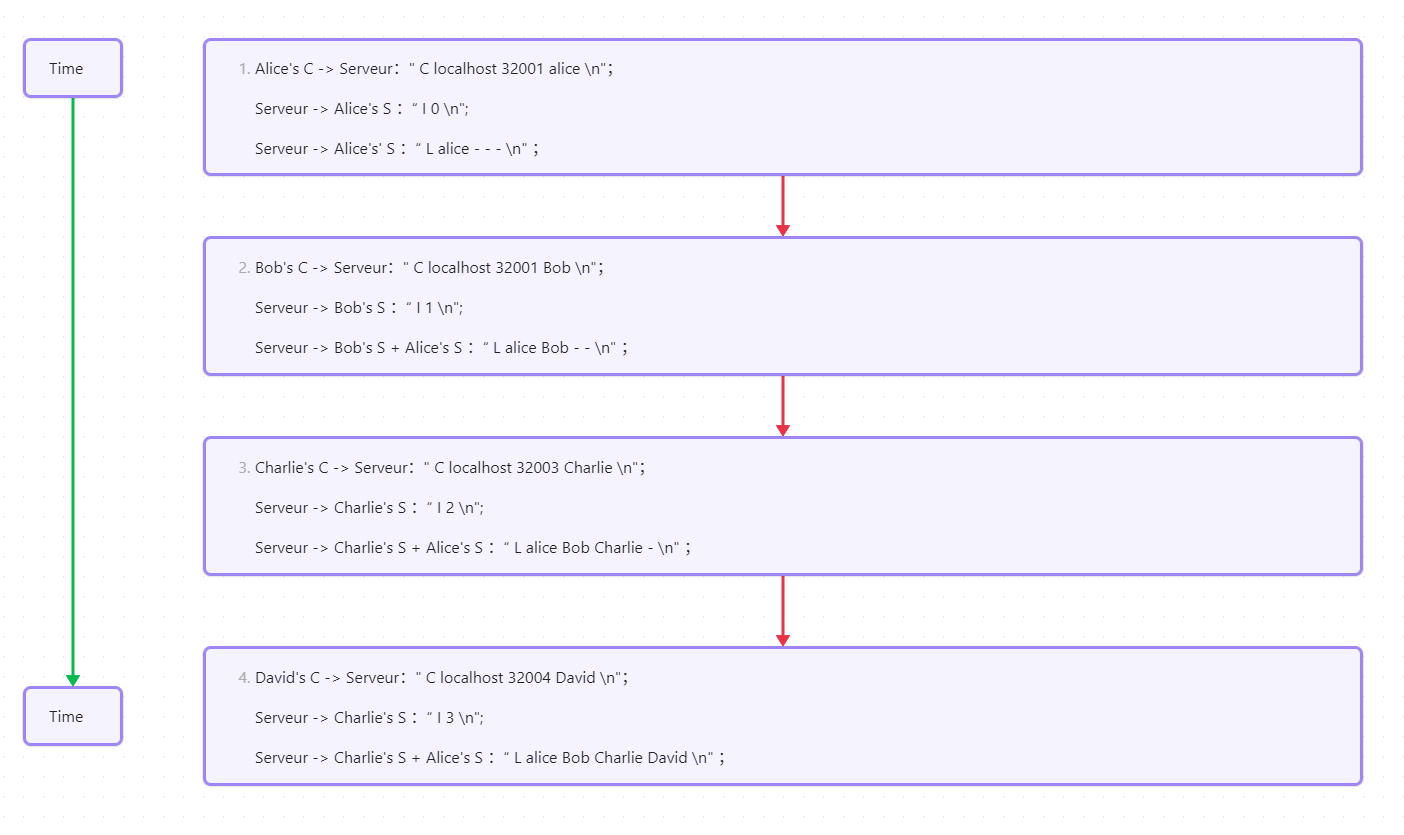
\includegraphics[width=0.95\linewidth]{images/Logique_de_connexion_des utilisateurs.PNG}
    \caption{Schéma illustrant la logique d'inscription des joueurs. Chaque client envoie son nom au serveur qui attribue un identifiant et renvoie à tous les autres la liste mise à jour.}
\end{figure}
    
Ce diagramme montre bien le fonctionnement du système de connexion. 
Le tout premier joueur envoie son nom, et le serveur lui répond avec une confirmation. 
Puis, au fur et à mesure que d'autres joueurs rejoignent, la liste des joueurs connectés est renvoyée à tous ceux qui sont déjà là. 
Ainsi, chaque client construit progressivement une vue complète de tous les participants.


\subsection{Partie client}

Le client communique avec le serveur en utilisant des sockets TCP également. 
Lors du démarrage, il se connecte à l'adresse IP et au port fournis, puis envoie les messages relatifs aux actions du joueur. 
La réception des messages du serveur est assurée par un fil séparé, ce qui permet à l'interface de continuer à répondre à l'utilisateur sans attendre les données réseau.

Ce client est composé de deux grandes parties : la logique du jeu et l'affichage graphique. 
La logique reçoit les informations, les interprète, les stocke dans des structures internes, puis demande à l'interface de se mettre à jour. 
L'interface graphique repose sur SDL2, une bibliothèque qui permet de créer des fenêtres, d'afficher des images et de gérer les clics et les mouvements de souris.

Les images sont chargées dès le lancement du jeu. 
Cela comprend les cartes, les icônes des symboles, les portraits, ainsi que les différents éléments de l'interface. 
Le joueur peut interagir avec le jeu en cliquant sur des zones de l'écran, comme les boutons qui permettent de choisir une action ou les zones représentant les cartes et les symboles. 
Une fois l'action choisie, l'information est transmise au serveur.

Une zone d'entrée permet également d'écrire son nom au début. 
Dès que le joueur rejoint la partie, il reçoit ses cartes, voit les symboles qui lui sont attribués, et suit le déroulement du tour grâce aux messages reçus. 
Il peut voir l'état des autres joueurs, leur statut (encore en jeu ou éliminé), et les résultats des actions en cours.

Le code utilise un verrou pour protéger certaines variables qui sont partagées entre les deux fils, comme le message reçu ou les résultats d'une question. 
Une petite variable de type indicateur permet aussi de prévenir l'interface quand une nouvelle information a été reçue, sans avoir à surveiller constamment l'arrivée de données.

La structure du client permet également de lancer le jeu avec différentes options, comme indiquer l'adresse du serveur, le port à utiliser, et le nom du joueur. 
En détectant la quantité d'informations saisies au démarrage du programme, 
le programme peut déterminer automatiquement la méthode que le joueur souhaite utiliser pour démarrer le programme client, 
aidant ainsi le joueur à commencer à jouer rapidement et facilement.

\begin{figure}[H]
    \centering
    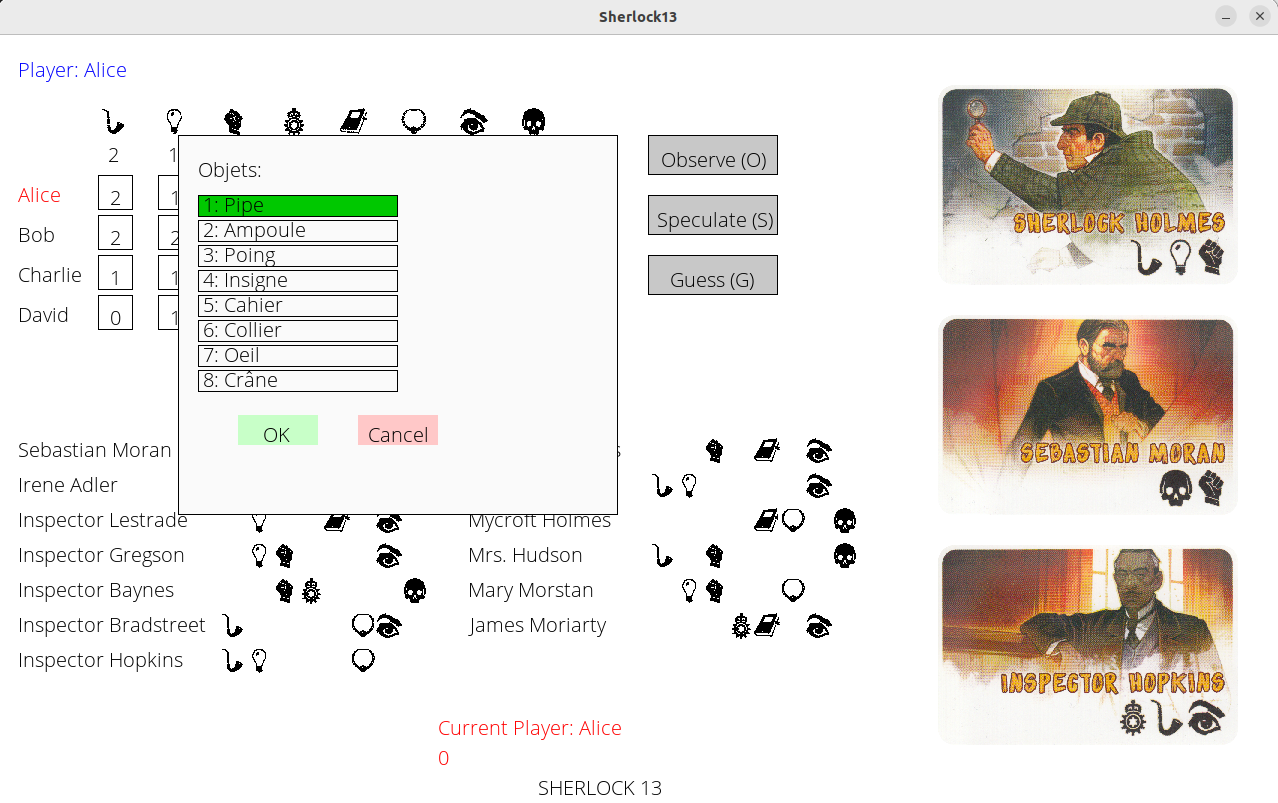
\includegraphics[width=0.3\linewidth]{images/Button_O.png}
    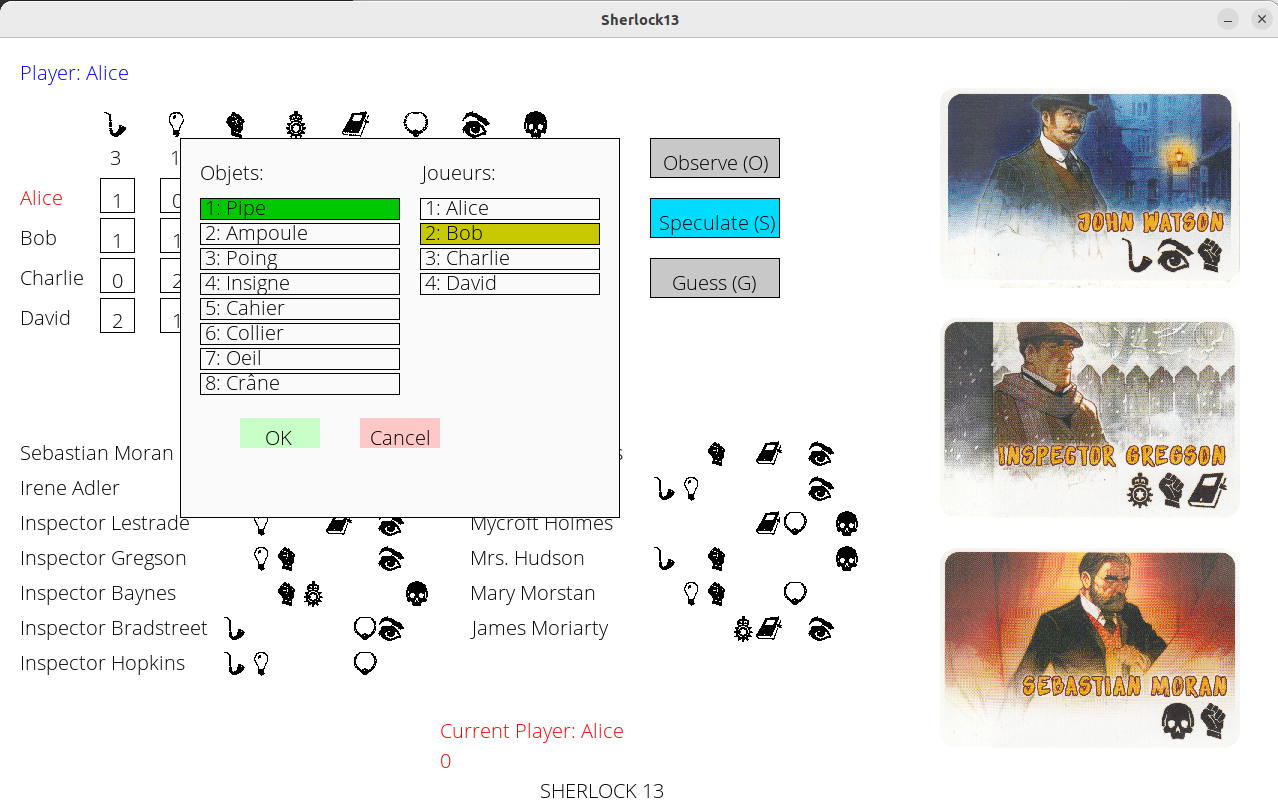
\includegraphics[width=0.3\linewidth]{images/Button_S.png}
    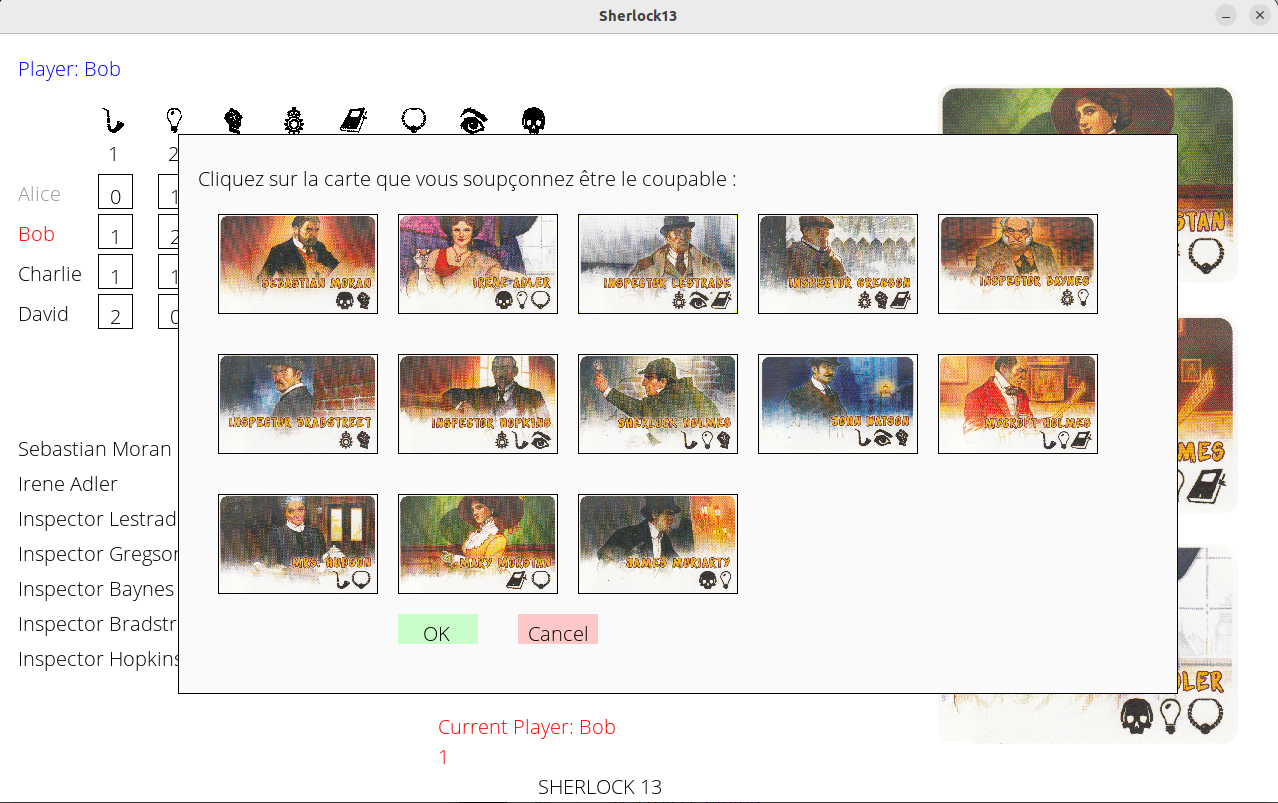
\includegraphics[width=0.3\linewidth]{images/Button_G.png}
    \caption{Ces trois boutons permettent au joueur d'interagir avec le jeu : observer un symbole, poser une question ciblée, ou faire une accusation.}
\end{figure}
    
Une fois cliqué, une fenêtre s'ouvrira pour spécifier le symbole ou le joueur concerné, permettant au joueur de terminer son opération.
    
\begin{figure}[H]
    \centering
    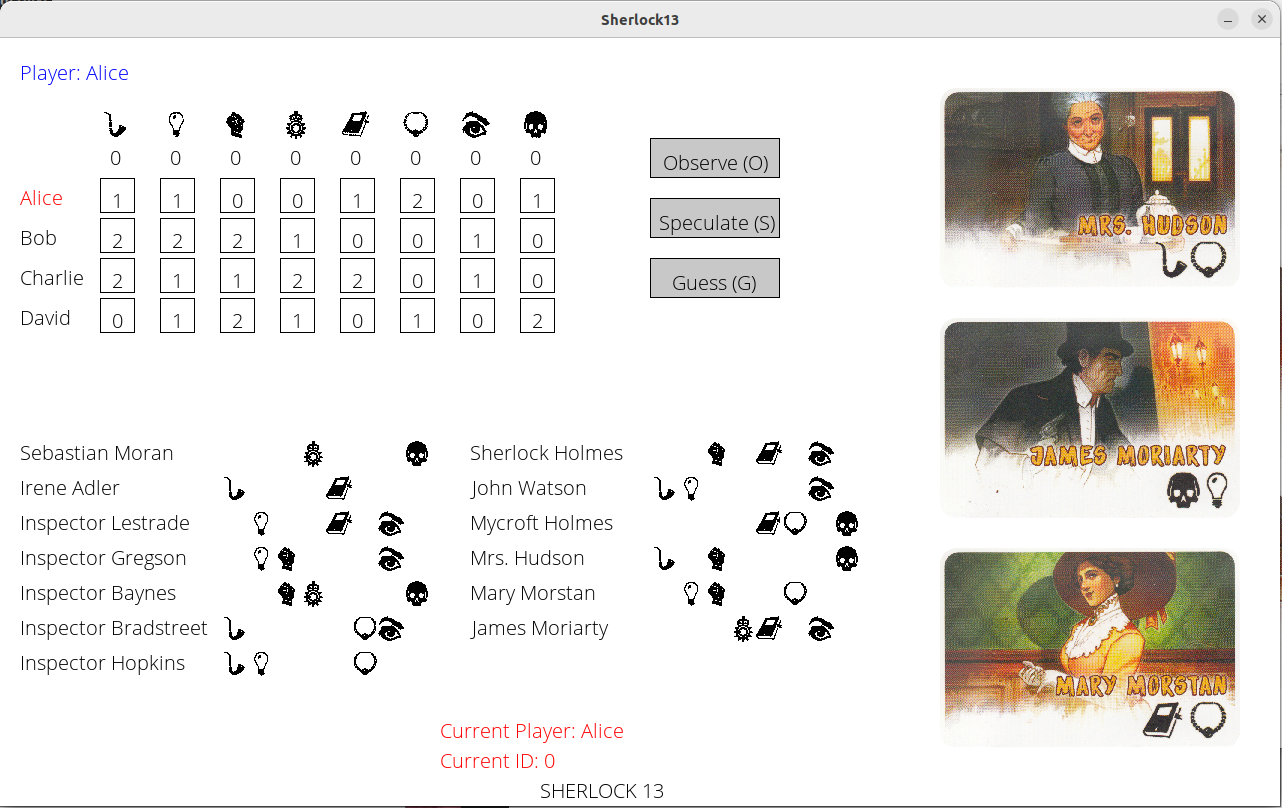
\includegraphics[width=0.95\linewidth]{images/Interface.png}
    \caption{Vue générale de l'interface graphique pendant une partie, avec les cartes affichées, les noms des joueurs, et le terminal en arrière-plan.}
\end{figure}
    
On peut voir ici comment le programme combine l'affichage graphique et le retour de la console. 
Les joueurs peuvent voir leurs noms dans le coin supérieur gauche de l'écran et quel joueur opère actuellement dans le coin inférieur de l'écran. 
Au milieu de l'écran se trouvent les boutons O, S et G.

\begin{figure}[H]
    \centering
    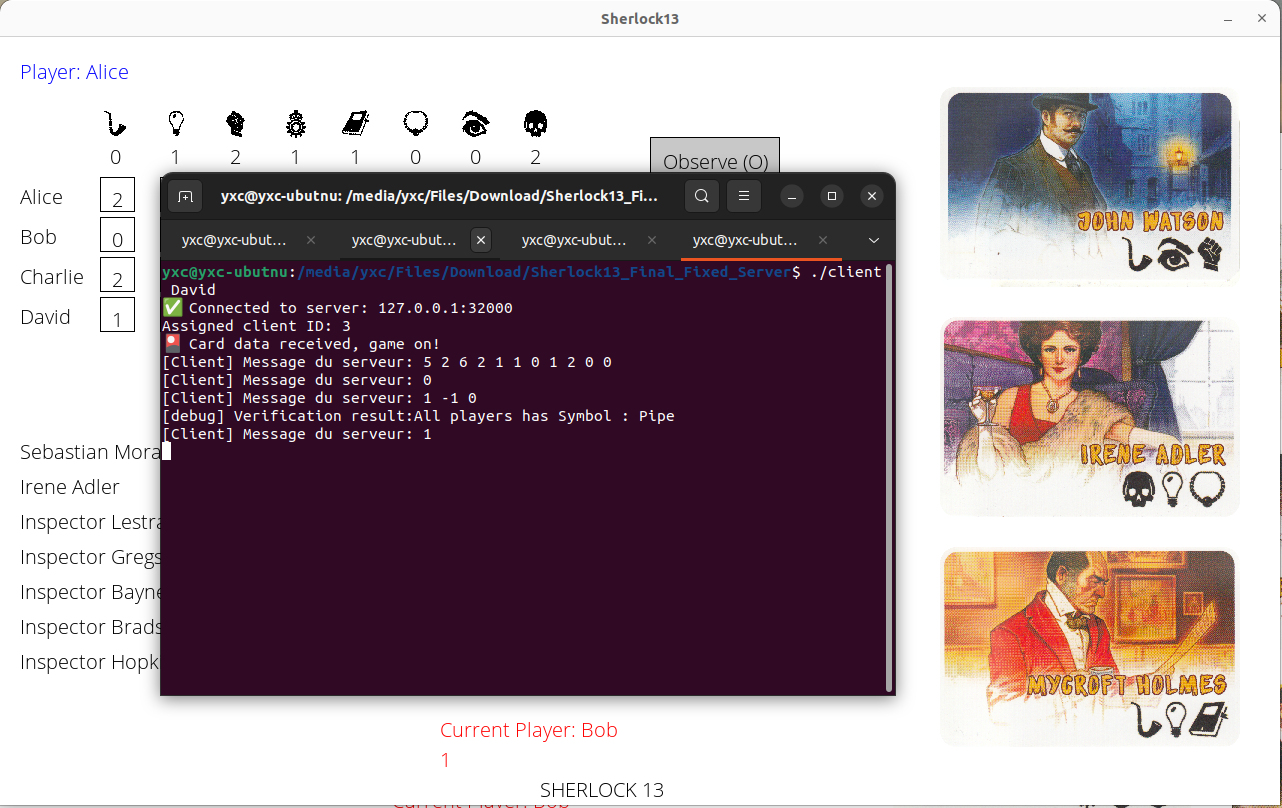
\includegraphics[width=0.9\linewidth]{images/message_returned.png}
    \caption{Réponse affichée après une question ouverte. Le serveur informe si le symbole demandé est visible chez les autres joueurs.}
\end{figure}
    
Lorsqu'un joueur clique sur le bouton “O” pour poser une question ouverte, il reçoit immédiatement une réponse du serveur. 
L'image montre les données renvoyées par le serveur.
    
\subsection{Considérations sur les processus et les pipes}

Dans l'architecture de ce projet, nous avons fait le choix d'utiliser des threads plutôt que des processus multiples avec pipes. 
Ce choix s'explique pour plusieurs raisons techniques liées à la structure du code et aux contraintes de la bibliothèque graphique.

Tout d'abord, du côté du client, il existe plusieurs données comme le tampon qui contient les messages réseau, 
l'identifiant du joueur et son nom. Ces informations doivent être accessibles à la fois par le fil qui reçoit les messages et par celui qui gère l'écran. 
Comme les deux partagent la même mémoire, les échanges sont simples et rapides. Si on utilisait deux processus différents, il faudrait trouver un moyen de copier toutes ces données entre eux, ce qui compliquerait le programme.

Ensuite, pour l'affichage, on utilise SDL qui impose que tout ce qui touche au dessin soit fait dans le fil principal. 
Si on séparait l'affichage et la communication réseau dans deux processus, il faudrait transmettre des instructions d'un à l'autre. 
Or SDL ne permet pas de partager un écran entre deux processus. Les threads permettent ici de rester dans le même contexte graphique sans problème.

Enfin, sur le serveur, toutes les informations sur les joueurs sont enregistrées dans un grand tableau accessible par tous les fils d'exécution. 
Grâce à cela, chaque action d'un joueur peut être traitée rapidement et les informations peuvent être mises à jour et transmises facilement. 
Si on avait utilisé un processus par connexion, il aurait fallu inventer un système pour partager ces données, ce qui aurait rendu le tout plus lent et plus fragile.

Il existe bien un moyen de communication entre processus, comme les tuyaux (ou pipes), 
qui permettent de transmettre un message dans un seul sens entre un programme parent et un programme fils. Voici un petit exemple :

\begin{texC}
int fd[2];
pipe(fd);
if (fork() == 0) {
    close(fd[1]);
    read(fd[0], buffer, sizeof(buffer));
} else {
    close(fd[0]);
    write(fd[1], "Message", 7);
}
\end{texC}

Mais ce mécanisme reste limité : il est plus adapté à des cas simples où un programme envoie des données à un autre sans attendre une réponse immédiate. 
Dans notre jeu, les messages vont et viennent rapidement, et ils doivent être traités presque tout de suite. Les threads permettent cela plus facilement.

En conclusion, pour ce projet, les threads sont plus adaptés : ils facilitent l'accès aux données, évitent les complications avec l'affichage, 
et permettent une gestion fluide et cohérente des joueurs. Les processus séparés et les pipes sont utiles dans d'autres situations, 
mais pas très fort pour ce type de jeu interactif en temps réel.

\section{Utilisation des concepts vus en TP}

Les sockets TCP sont utilisées pour transmettre les messages entre les clients et le serveur. 
Le serveur crée une socket, l'attache à un port, attend les connexions et reçoit les messages. 
Les clients se connectent temporairement pour envoyer leurs messages d'action. 
C'est comme ce qu'on a aprris pendent les TPs.

Les threads sont présents du côté client pour permettre l'exécution concurrente de l'interface graphique et de la réception des messages du serveur. 
Cela évite que l'application ne se bloque en attente de messages. 
La synchronisation est assurée par une variable partagée, protégée par un mutex pour garantir une lecture/écriture correcte.

Concernant les processus, même s'ils n'ont pas été directement utilisés dans ce projet, 
ils auraient pu servir pour décomposer les fonctionnalités du client en entités indépendantes, 
comme cela a été fait en TP avec l'utilisation de \texttt{fork()} et \texttt{exec()}.

Ils permettent une communication simple entre deux processus via un canal de type FIFO. 
Cela aurait pu remplacer les sockets dans un cas où tous les processus sont locaux.

\section{Conclusion}

Le projet Sherlock 13 implémente une architecture client-serveur avec une interface graphique, appliquant les connaissances acquises au travail réel. 
Les principaux défis concernent la synchronisation entre les threads, la gestion des messages et les structures de données. 
Grâce à ce projet, j'ai approfondi ma compréhension des sockets, des communications réseau et de la programmation simultanée. 
J'ai pleinement expérimenté le rôle des verrous mutex et des multi-processus dans les tests, 
compris les problèmes qui peuvent être rencontrés lors de la synchronisation entre les threads et appris et utilisé la bibliothèque graphique SDL2.

\end{document}

